\begin{figure*}[t]
\centering
\definecolor{coHubFill}{HTML}{1B365D}
\definecolor{coHubBorder}{HTML}{102340}
\definecolor{coHubHalo}{HTML}{EBF1F8}
\definecolor{coHubHaloLine}{HTML}{9BB0C7}
\definecolor{coHubSub}{HTML}{D8E4F2}
\definecolor{coInk}{HTML}{1C2D40}
\definecolor{coMuted}{HTML}{4F6275}
\definecolor{coStroke}{HTML}{476078}
\definecolor{coReadLine}{HTML}{8196AC}
\definecolor{coNodeFill}{HTML}{F9FBFD}
\definecolor{coBriefFill}{HTML}{F2F5F8}
\definecolor{coDetectFill}{HTML}{EEF3F8}
\definecolor{coTermFill}{HTML}{E3ECF4}
\definecolor{coTermBorder}{HTML}{2A4A6E}
\pgfdeclarelayer{bg}
\pgfsetlayers{bg,main}
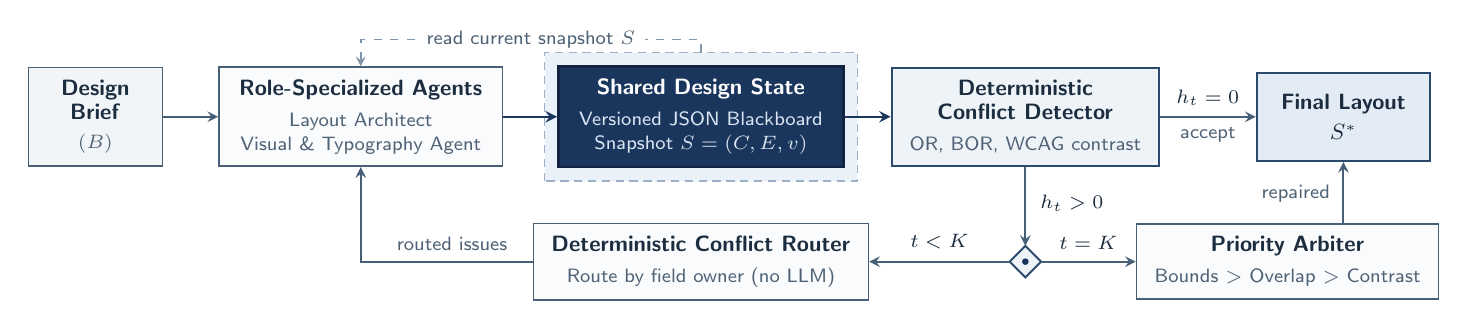
\begin{tikzpicture}[
    x=1cm, y=1cm, font=\sffamily\fontsize{7.6}{9.2}\selectfont,
    boxbase/.style={align=center, inner xsep=6.5pt, inner ysep=4.5pt},
    briefbox/.style={boxbase, draw=coStroke, fill=coBriefFill,
        text=coInk, line width=.58pt, minimum height=1.12cm},
    process/.style={boxbase, draw=coStroke, fill=coNodeFill,
        text=coInk, line width=.62pt, minimum height=1.12cm},
    detectorbox/.style={boxbase, draw=coTermBorder, fill=coDetectFill,
        text=coInk, line width=.68pt, minimum height=1.12cm},
    hubbox/.style={boxbase, draw=coHubBorder, fill=coHubFill,
        text=white, line width=.95pt, minimum height=1.16cm,
        inner xsep=7.5pt, inner ysep=4.6pt},
    terminal/.style={boxbase, draw=coTermBorder, fill=coTermFill,
        text=coInk, line width=.78pt, minimum height=1.12cm},
    flow/.style={draw=coStroke, line width=.70pt, ->, >=stealth},
    hubflow/.style={draw=coHubFill, line width=.85pt, ->, >=stealth},
    readflow/.style={draw=coReadLine, line width=.56pt, dashed, ->, >=stealth},
    cond/.style={font=\sffamily\fontsize{7}{8.2}\selectfont,
        text=coInk, inner sep=1.6pt},
    note/.style={font=\sffamily\fontsize{7}{8.2}\selectfont,
        text=coMuted, inner sep=1.5pt},
    badge/.style={font=\sffamily\fontsize{7}{8.2}\selectfont,
        text=coMuted, fill=white, inner xsep=3.5pt, inner ysep=1.2pt},
]
% Row 1: Brief -> Agents -> Shared Design State (Hub) -> Detector -> Unified Final Layout.
\node[briefbox, minimum width=1.70cm] (brief) at (0.85,0)
    {\textbf{Design}\\[-0.5pt]\textbf{Brief}\\[1.5pt]%
     {\fontsize{7}{8.0}\selectfont\color{coMuted}$(B)$}};
\node[process, minimum width=3.60cm] (agents) at (4.22,0)
    {\textbf{Role-Specialized Agents}\\[2pt]%
     {\fontsize{6.9}{8.2}\selectfont\color{coMuted}Layout Architect}\\[-0.5pt]%
     {\fontsize{6.9}{8.2}\selectfont\color{coMuted}Visual \& Typography Agent}};
\node[hubbox, minimum width=3.40cm] (board) at (8.54,0)
    {\textbf{Shared Design State}\\[2pt]%
     {\fontsize{6.9}{8.2}\selectfont\color{coHubSub}Versioned JSON Blackboard}\\[-0.5pt]%
     {\fontsize{7}{8.2}\selectfont\color{coHubSub}Snapshot $S=(C,E,v)$}};
\node[detectorbox, minimum width=3.20cm] (detector) at (12.66,0)
    {\textbf{Deterministic}\\[-0.5pt]\textbf{Conflict Detector}\\[2pt]%
     {\fontsize{6.9}{8.2}\selectfont\color{coMuted}OR, BOR, WCAG contrast}};
\node[terminal, minimum width=2.20cm] (final) at (16.70,0)
    {\textbf{Final Layout}\\[1.5pt]\textbf{$S^{*}$}};

% Sharp orthogonal outer frame highlighting Shared Design State as the central hub.
\begin{pgfonlayer}{bg}
\fill[coHubHalo]
    ([xshift=-4.5pt,yshift=-4.5pt]board.south west) rectangle
    ([xshift=4.5pt,yshift=4.5pt]board.north east);
\draw[coHubHaloLine, line width=.48pt, densely dashed]
    ([xshift=-4.5pt,yshift=-4.5pt]board.south west) rectangle
    ([xshift=4.5pt,yshift=4.5pt]board.north east);
\end{pgfonlayer}

% Primary Row-1 flow.
\draw[flow] (brief.east) -- (agents.west);
\draw[hubflow] (agents.east) -- (board.west);
\draw[hubflow] (board.east) -- (detector.west);
\draw[flow] (detector.east) --
    node[cond,above=2pt] {$h_t=0$}
    node[note,below=2pt] {accept}
    (final.west);

% Orthogonal blackboard read-back path above Row 1.
\draw[readflow]
    ([yshift=4.5pt]board.north) -- (8.54,0.98) --
    node[badge] {read current snapshot $S$}
    (4.22,0.98) -- (agents.north);

% Row 2: Router (aligned under Hub), Decision Diamond (under Detector), Priority Arbiter.
\node[process, minimum width=3.95cm, minimum height=0.86cm] (critic) at (8.54,-1.84)
    {\textbf{Deterministic Conflict Router}\\[2pt]%
     {\fontsize{6.8}{8.2}\selectfont\color{coMuted}Route by field owner (no LLM)}};
\node[process, minimum width=3.62cm, minimum height=0.86cm] (arbiter) at (15.99,-1.84)
    {\textbf{Priority Arbiter}\\[2pt]%
     {\fontsize{7}{8.2}\selectfont\color{coMuted}Bounds $>$ Overlap $>$ Contrast}};

% Centered decision diamond directly beneath the deterministic conflict detector.
\coordinate (fork) at (12.66,-1.84);
\coordinate (forkN) at (12.66,-1.64);
\coordinate (forkS) at (12.66,-2.04);
\coordinate (forkW) at (12.46,-1.84);
\coordinate (forkE) at (12.86,-1.84);

\draw[flow] (detector.south) --
    node[cond,right=3.5pt,pos=0.46] {$h_t>0$}
    (forkN);
\fill[coDetectFill] (forkN) -- (forkE) -- (forkS) -- (forkW) -- cycle;
\draw[coTermBorder, line width=.70pt] (forkN) -- (forkE) -- (forkS) -- (forkW) -- cycle;
\fill[coHubFill] (fork) circle (1.2pt);

% Branch routing: iterative refinement (t < K) vs. fallback repair merging into Final Layout S*.
\draw[flow] (forkW) -- node[cond,above=2.5pt] {$t<K$} (critic.east);
\draw[flow] (critic.west) -| (agents.south);
\node[note, above=2.5pt] at (5.38,-1.84) {routed issues};
\draw[flow] (forkE) -- node[cond,above=2.5pt] {$t=K$} (arbiter.west);
\draw[flow] (final.south |- arbiter.north) --
    node[note,left=3pt,pos=0.48] {repaired}
    (final.south);
\end{tikzpicture}
\caption{CoLayout control flow. At the start of correction round $t$, the detector counts
$h_t$ hard conflicts on the latest state. The deterministic router dispatches unresolved conflicts
to their field owners (no extra LLM call) while rounds remain. At the round budget $K$, the arbiter applies
repairs in priority order.}
\label{fig:architecture}
\end{figure*}
